%% Supplementary material
\documentclass{article}\usepackage[]{graphicx}\usepackage[]{color}
%% maxwidth is the original width if it is less than linewidth
%% otherwise use linewidth (to make sure the graphics do not exceed the margin)
\makeatletter
\def\maxwidth{ %
  \ifdim\Gin@nat@width>\linewidth
    \linewidth
  \else
    \Gin@nat@width
  \fi
}
\makeatother

\definecolor{fgcolor}{rgb}{0.345, 0.345, 0.345}
\newcommand{\hlnum}[1]{\textcolor[rgb]{0.686,0.059,0.569}{#1}}%
\newcommand{\hlstr}[1]{\textcolor[rgb]{0.192,0.494,0.8}{#1}}%
\newcommand{\hlcom}[1]{\textcolor[rgb]{0.678,0.584,0.686}{\textit{#1}}}%
\newcommand{\hlopt}[1]{\textcolor[rgb]{0,0,0}{#1}}%
\newcommand{\hlstd}[1]{\textcolor[rgb]{0.345,0.345,0.345}{#1}}%
\newcommand{\hlkwa}[1]{\textcolor[rgb]{0.161,0.373,0.58}{\textbf{#1}}}%
\newcommand{\hlkwb}[1]{\textcolor[rgb]{0.69,0.353,0.396}{#1}}%
\newcommand{\hlkwc}[1]{\textcolor[rgb]{0.333,0.667,0.333}{#1}}%
\newcommand{\hlkwd}[1]{\textcolor[rgb]{0.737,0.353,0.396}{\textbf{#1}}}%

\usepackage{framed}
\makeatletter
\newenvironment{kframe}{%
 \def\at@end@of@kframe{}%
 \ifinner\ifhmode%
  \def\at@end@of@kframe{\end{minipage}}%
  \begin{minipage}{\columnwidth}%
 \fi\fi%
 \def\FrameCommand##1{\hskip\@totalleftmargin \hskip-\fboxsep
 \colorbox{shadecolor}{##1}\hskip-\fboxsep
     % There is no \\@totalrightmargin, so:
     \hskip-\linewidth \hskip-\@totalleftmargin \hskip\columnwidth}%
 \MakeFramed {\advance\hsize-\width
   \@totalleftmargin\z@ \linewidth\hsize
   \@setminipage}}%
 {\par\unskip\endMakeFramed%
 \at@end@of@kframe}
\makeatother

\definecolor{shadecolor}{rgb}{.97, .97, .97}
\definecolor{messagecolor}{rgb}{0, 0, 0}
\definecolor{warningcolor}{rgb}{1, 0, 1}
\definecolor{errorcolor}{rgb}{1, 0, 0}
\newenvironment{knitrout}{}{} % an empty environment to be redefined in TeX

\usepackage{alltt}

%% Load required packages
\usepackage{amsmath,amsfonts,bm}
\usepackage[round]{natbib}
\usepackage{hyperref}

%% Macros
\newcommand{\trans}{\ensuremath{^\prime}}
\newcommand{\boot}{\star} % or possiibly *
%\newcommand{\code}[1]{\texttt{\small{#1}}}
%\newcommand{\pkg}[1]{\textsf{\small{#1}}}
\newcommand{\proglang}[1]{\textsf{#1}}
\newcommand{\code}[1]{\texttt{#1}}
\newcommand{\pkg}[1]{\textsf{#1}}\newcommand{\var}{\ensuremath{\mathbb{V}}}
\newcommand{\se}{\ensuremath{\mathrm{se}}}
\newcommand{\E}{\ensuremath{\mathbb{E}}}
\newcommand{\X}{\ensuremath{\bm{X}}}
\newcommand{\Z}{\ensuremath{\bm{Z}}}
\newcommand{\newln}{\\&\quad\quad\quad\quad{}}
\newtheorem{rexample}{R Example}%[section]

%% Title
\title{Web-based Supplementary Materials for "Linear Calibration with Grouped Data" by Brandon M. Greenwell and Christine M. Schubert}
\date{}
\author{}
\IfFileExists{upquote.sty}{\usepackage{upquote}}{}

\begin{document}

\maketitle




\section*{Web Appendix A}
\subsection*{The ML Estimator of $x_0$ for the Random Intercept Model}

%Put your short appendix here.  Remember, longer appendices are
%possible when presented as Supplementary Web Material.  Please 
%review and follow the journal policy for this material, available
%under Instructions for Authors at \texttt{http://www.biometrics.tibs.org}.

In this appendix, we show that the inverse estimator, $\widehat{x}_0 = \mu^{-1}\left(\mathcal{Y}_0; \widehat{\bm{\beta}}\right)$, is the ML estimator of $x_0$ for the random intercept model. For this model, note that the scaled variance-covariance matrix of the random effect becomes $\bm{G}^\dagger = \tau\bm{I}$ and that $\Z_i = \bm{1}_i$ (a column vector of all ones), hence, $\bm{V}_i = \sigma_\epsilon^2\left(\bm{I}_i + \tau\bm{J}_i\right)$ where $\bm{J}_i = \bm{1}_i\bm{1}_i\trans$. Therefore, we can write
\[
  \bm{\mathcal{Y}}_i \sim \mathcal{N}\left\{\X_i\bm{\beta}, \sigma_\epsilon^2\left(\bm{I}_i + \tau\bm{J}_i\right)\right\}, \quad i = 1, \dotsc, m,
\]
where $\X_i$ is an $n_i \times 2$ design matrix with $j$-th row equal to $\X_{ij}\trans = \left(1, x_{ij}\right)$, $\bm{\beta} = \left(\beta_0, \beta_1\right)\trans$ is a vector of fixed effects, $\sigma_\epsilon^2$ is the within-subject variance, and $\sigma_\epsilon^2\tau$ is the variance of the random intercepts. Ignoring constants, the log-likelihood for the data is
\begin{multline*}
  \ell_{\mathrm{I}}\left(\bm{\beta}, \sigma_\epsilon^2, \tau\right) = -\frac{N}{2}\log\left(\sigma_\epsilon^2\right) - \frac{1}{2}\sum_{i = 1}^m \log\left|\bm{I} + \tau\bm{J}_i\right| \\ - \frac{1}{2\sigma_\epsilon^2}\sum_{i = 1}^m \left(\bm{\mathcal{Y}}_i - \X_i\bm{\beta}\right)\trans\left(\bm{I} + \tau\bm{J}_i\right)^{-1}\left(\bm{\mathcal{Y}}_i - \X_i\bm{\beta}\right).
\end{multline*}
The subscript "$\mathrm{I}$" is there to remind us that this is the likelihood for the data from the first stage of the calibration experiment. Using the following formulas \citep[pg. 49]{demidenko_mixed_2013},
\begin{itemize}
  \item $\left|\bm{I} + \tau\bm{J}_i\right| = 1 + n_i\tau$;
  \item $\left(\bm{I} + \tau\bm{J}_i\right)^{-1} = \bm{I} - \frac{\tau}{1 + n_i\tau}\bm{J}_i$;
\end{itemize}
the log-likelihood simplifies to
\begin{multline*}
  \ell_{\mathrm{I}}\left(\bm{\beta}, \sigma_\epsilon^2, \tau\right) = -\frac{N}{2}\log\left(\sigma_\epsilon^2\right) - \frac{1}{2}\sum_{i = 1}^m \log\left(1 + n_i\tau\right) \\ - \frac{1}{2\sigma_\epsilon^2}\sum_{i = 1}^m \left(\bm{\mathcal{Y}}_i - \X_i\bm{\beta}\right)\trans\left(\bm{I} - \frac{\tau}{1 + n_i\tau}\bm{J}_i\right)\left(\bm{\mathcal{Y}}_i - \X_i\bm{\beta}\right).
\end{multline*}
Similarly, the log-likelihood for $\mathcal{Y}_0$ (i.e., the data from the second stage of the calibration experiment) is 
\[
  \mathcal{\ell}_{\mathrm{II}}\left(\bm{\beta}, \sigma_\epsilon^2, \tau, x_0\right) = -\frac{1}{2}\log\left(\sigma_\epsilon^2\right) - \frac{1}{2}\log\left(1 + \tau\right) - \frac{1}{2\sigma_\epsilon^2\left(1 + \tau\right)}\left(\mathcal{Y}_0 - \beta_0 - \beta_1 x_0\right)^2.
\]
From the independence of $\bm{\mathcal{Y}}$ and $\mathcal{Y}_0$, the log-likelihood for the pooled data, denoted $\mathcal{\ell}\left(\bm{\beta}, \sigma_\epsilon^2, \tau, x_0\right)$, is given by
\begin{align*}
  \ell\left(\bm{\beta}, \sigma_\epsilon^2, \tau, x_0\right) &= \mathcal{\ell}_{\mathrm{I}}\left(\bm{\beta}, \sigma_\epsilon^2, \tau\right) + \mathcal{\ell}_{\mathrm{II}}\left(\bm{\beta}, \sigma_\epsilon^2, \tau, x_0\right) \\
  &= -\frac{N+1}{2}\log\left(\sigma_\epsilon^2\right) - \frac{1}{2}\sum_{i = 1}^m \log\left(1 + n_i\tau\right) - \frac{1}{2}\log\left(1 + \tau\right) \newln - \frac{1}{2\sigma_\epsilon^2}\sum_{i = 1}^m \left(\bm{\mathcal{Y}}_i - \X_i\bm{\beta}\right)\trans\left(\bm{I} - \frac{\tau}{1 + n_i\tau}\bm{J}_i\right)\left(\bm{\mathcal{Y}}_i - \X_i\bm{\beta}\right) \newln - \frac{1}{2\sigma_\epsilon^2\left(1 + \tau\right)}\left(\mathcal{Y}_0 - \beta_0 - \beta_1 x_0\right)^2.
\end{align*}
Thus, the full log-likelihood is the sum of two parts, the log-likelihood for the standards, and the log-likelihood for the unknown. Equating to zero the partial derivative of the full log-likelihood with respect to the parameter $x_0$ results in $\widetilde{x}_0\left(\bm{\beta}\right) = \left(\mathcal{Y}_0 - \beta_0\right)/\beta_1$. In other words, for any value of $\bm{\beta}$, $\widetilde{x}_0\left(\bm{\beta}\right)$ maximizes the likelihood with respect to $x_0$. Substituting this into the log-likelihood yields the \textit{profiled log-likelihood}
\begin{multline*}
  \mathcal{\ell}_p\left(\bm{\beta}, \sigma_\epsilon^2, \tau\right) = -\frac{N+1}{2}\log\left(\sigma_\epsilon^2\right) - \frac{1}{2}\sum_{i = 1}^m \log\left(1 + n_i\tau\right) - \frac{1}{2}\log\left(1 + \tau\right) \\ - \frac{1}{2\sigma_\epsilon^2}\sum_{i = 1}^m \left(\bm{\mathcal{Y}}_i - \X_i\bm{\beta}\right)\trans\left(\bm{I} - \frac{\tau}{1 + n_i\tau}\bm{J}_i\right)\left(\bm{\mathcal{Y}}_i - \X_i\bm{\beta}\right),
\end{multline*}
Similarly, equating the partial derivative of $\mathcal{\ell}_p\left(\bm{\beta}, \sigma_\epsilon^2, \tau\right)$, with respect to the parameter $\sigma_\epsilon^2$, to zero yields 
\[
  \widetilde{\sigma}_\epsilon^2\left(\bm{\beta}, \tau\right) = \frac{1}{N + 1}\sum_{i = 1}^m \left(\bm{\mathcal{Y}}_i - \X_i\bm{\beta}\right)\left(\bm{I} - \frac{\tau}{1 + n_i\tau}\bm{J}_i\right)\left(\bm{\mathcal{Y}}_i - \X_i\bm{\beta}\right)\trans.
\]
Substituting this into the profiled log-likelihood and simplifying we get
\begin{multline*}
  \mathcal{\ell}_p\left(\bm{\beta}, \tau\right) = -\frac{N+1}{2}\log\left\{\sum_{i = 1}^m \left(\bm{\mathcal{Y}}_i - \X_i\bm{\beta}\right)\trans\left(\bm{I} - \frac{\tau}{1 + n_i\tau}\bm{J}_i\right)\left(\bm{\mathcal{Y}}_i - \X_i\bm{\beta}\right)\right\} \\ - \frac{1}{2}\sum_{i = 1}^m \log\left(1 + n_i\tau\right) - \frac{1}{2}\log\left(1 + \tau\right),
\end{multline*}
The parameters $x_0$ and $\sigma_\epsilon^2$ have been "profiled out", resulting in a simpler log-likelihood in only $p + 1$ parameters. We could continue in this fashion with the parameter $\bm{\beta}$ as well, although, it is quite easy to see that the value of $\bm{\beta}$ that maximizes $\mathcal{\ell}_p\left(\bm{\beta}, \tau\right)$ is just the usual generalized least squares estimator, $\widetilde{\bm{\beta}}\left(\tau\right)$. Furthermore, it can be shown \citep{demidenko_mixed_2013} that, for the balanced case, $\widetilde{\bm{\beta}}\left(\tau\right) = \widetilde{\bm{\beta}}$ does not depend on $\tau$ and in fact reduces to the ordinary least squares estimator $\widehat{\bm{\beta}} = \left(\X\trans\X\right)^{-1}\X\trans\bm{\mathcal{Y}}$. Thus, the ML estimator of $x_0$ for the balanced random intercept model is simply
\[
  \widehat{x}_0 = \widetilde{x}_0\left(\widehat{\bm{\beta}}\right) = \frac{\mathcal{Y}_0 - \widehat{\beta}_0}{\widehat{\beta}_1},
\]
where 
\[
  \widehat{\beta}_1 = \frac{\sum_{i=1}^n\sum_{j=1}^m\left(x_{ij}-\bar{x}\right)\left(y_{ij}-\bar{y}\right)}{\sum_{i=1}^n\sum_{j=1}^m\left(x_{ij}-\bar{x}\right)^2}, \quad \widehat{\beta}_0 = \bar{y} - \widehat{\beta}_1\bar{x}.
\]

\section*{Web Appendix B}
\subsection*{Example \proglang{R} code}

The following snippets of \proglang{R} code are provided as a template for implementing the various methods outlined in our paper. The first example loads the necessary packages and data, and fits the LMM discussed in the paper.
\begin{knitrout}
\definecolor{shadecolor}{rgb}{0.969, 0.969, 0.969}\color{fgcolor}\begin{kframe}
\begin{rexample}\label{example-1}\hfill{}\begin{alltt}
\hlcom{## Load packages}
\hlkwd{library}\hlstd{(car)}  \hlcom{# for deltaMethod() function}
\hlkwd{library}\hlstd{(nlme)}  \hlcom{# for fitting LMMs}
\hlkwd{library}\hlstd{(lme4)}  \hlcom{# for fitting LMMs and parametric bootstrap}
\hlkwd{library}\hlstd{(boot)}  \hlcom{# for calculating bootstrap CI's}


\hlcom{## Bladder data}
\hlstd{subject} \hlkwb{<-} \hlkwd{rep}\hlstd{(}\hlnum{1}\hlopt{:}\hlnum{23}\hlstd{,} \hlkwc{times} \hlstd{=} \hlnum{8}\hlstd{)}
\hlstd{volume} \hlkwb{<-} \hlkwd{rep}\hlstd{(}\hlkwd{c}\hlstd{(}\hlnum{10}\hlstd{,} \hlnum{25}\hlstd{,} \hlnum{50}\hlstd{,} \hlnum{75}\hlstd{,} \hlnum{100}\hlstd{,} \hlnum{125}\hlstd{,} \hlnum{150}\hlstd{,} \hlnum{175}\hlstd{),}
    \hlkwc{each} \hlstd{=} \hlnum{23}\hlstd{)}
\hlstd{HD} \hlkwb{<-} \hlkwd{c}\hlstd{(}\hlnum{13.2}\hlstd{,} \hlnum{11.1}\hlstd{,} \hlnum{10.3}\hlstd{,} \hlnum{NA}\hlstd{,} \hlnum{4.8}\hlstd{,} \hlnum{7.7}\hlstd{,} \hlnum{NA}\hlstd{,} \hlnum{5.9}\hlstd{,} \hlnum{1.9}\hlstd{,}
    \hlnum{6.5}\hlstd{,} \hlnum{19.8}\hlstd{,} \hlnum{14.6}\hlstd{,} \hlnum{NA}\hlstd{,} \hlnum{NA}\hlstd{,} \hlnum{9.7}\hlstd{,} \hlnum{17.2}\hlstd{,} \hlnum{10.6}\hlstd{,} \hlnum{19.3}\hlstd{,}
    \hlnum{8.5}\hlstd{,} \hlnum{6.9}\hlstd{,} \hlnum{8.1}\hlstd{,} \hlnum{14.8}\hlstd{,} \hlnum{13.7}\hlstd{,} \hlnum{27.4}\hlstd{,} \hlnum{27.5}\hlstd{,} \hlnum{15}\hlstd{,} \hlnum{10}\hlstd{,}
    \hlnum{18.6}\hlstd{,} \hlnum{12.6}\hlstd{,} \hlnum{24}\hlstd{,} \hlnum{28.4}\hlstd{,} \hlnum{12.5}\hlstd{,} \hlnum{16.7}\hlstd{,} \hlnum{29.6}\hlstd{,} \hlnum{27.1}\hlstd{,} \hlnum{14}\hlstd{,}
    \hlnum{18.7}\hlstd{,} \hlnum{20.3}\hlstd{,} \hlnum{35.8}\hlstd{,} \hlnum{23.6}\hlstd{,} \hlnum{37.4}\hlstd{,} \hlnum{31.3}\hlstd{,} \hlnum{23.7}\hlstd{,} \hlnum{22}\hlstd{,} \hlnum{34.3}\hlstd{,}
    \hlnum{28.5}\hlstd{,} \hlnum{41.6}\hlstd{,} \hlnum{58.1}\hlstd{,} \hlnum{34.2}\hlstd{,} \hlnum{28.8}\hlstd{,} \hlnum{29.9}\hlstd{,} \hlnum{31.4}\hlstd{,} \hlnum{46.9}\hlstd{,}
    \hlnum{44.4}\hlstd{,} \hlnum{26.8}\hlstd{,} \hlnum{30.6}\hlstd{,} \hlnum{51.7}\hlstd{,} \hlnum{49.8}\hlstd{,} \hlnum{19.1}\hlstd{,} \hlnum{35.8}\hlstd{,} \hlnum{38.9}\hlstd{,}
    \hlnum{41.4}\hlstd{,} \hlnum{49.9}\hlstd{,} \hlnum{58.6}\hlstd{,} \hlnum{54.8}\hlstd{,} \hlnum{44}\hlstd{,} \hlnum{39.1}\hlstd{,} \hlnum{58.5}\hlstd{,} \hlnum{41.5}\hlstd{,} \hlnum{60.1}\hlstd{,}
    \hlnum{78.8}\hlstd{,} \hlnum{49.4}\hlstd{,} \hlnum{46.4}\hlstd{,} \hlnum{39.4}\hlstd{,} \hlnum{45.3}\hlstd{,} \hlnum{50.4}\hlstd{,} \hlnum{70.7}\hlstd{,} \hlnum{54.4}\hlstd{,}
    \hlnum{41.8}\hlstd{,} \hlnum{72.2}\hlstd{,} \hlnum{67.5}\hlstd{,} \hlnum{39.2}\hlstd{,} \hlnum{49.6}\hlstd{,} \hlnum{65.1}\hlstd{,} \hlnum{69.7}\hlstd{,} \hlnum{67.7}\hlstd{,}
    \hlnum{73.7}\hlstd{,} \hlnum{78.3}\hlstd{,} \hlnum{65.7}\hlstd{,} \hlnum{44.7}\hlstd{,} \hlnum{72.1}\hlstd{,} \hlnum{59.8}\hlstd{,} \hlnum{73.9}\hlstd{,} \hlnum{91.5}\hlstd{,}
    \hlnum{71.3}\hlstd{,} \hlnum{54.8}\hlstd{,} \hlnum{NA}\hlstd{,} \hlnum{48}\hlstd{,} \hlnum{67.8}\hlstd{,} \hlnum{89.4}\hlstd{,} \hlnum{63.1}\hlstd{,} \hlnum{49.6}\hlstd{,} \hlnum{81.9}\hlstd{,}
    \hlnum{79.1}\hlstd{,} \hlnum{48.7}\hlstd{,} \hlnum{65.6}\hlstd{,} \hlnum{65.1}\hlstd{,} \hlnum{81.9}\hlstd{,} \hlnum{87.7}\hlstd{,} \hlnum{79.4}\hlstd{,} \hlnum{93}\hlstd{,} \hlnum{80.3}\hlstd{,}
    \hlnum{68.9}\hlstd{,} \hlnum{90.9}\hlstd{,} \hlnum{77.5}\hlstd{,} \hlnum{85.5}\hlstd{,} \hlnum{98.3}\hlstd{,} \hlnum{81.3}\hlstd{,} \hlnum{69.4}\hlstd{,} \hlnum{NA}\hlstd{,} \hlnum{66.6}\hlstd{,}
    \hlnum{81}\hlstd{,} \hlnum{105.8}\hlstd{,} \hlnum{83.5}\hlstd{,} \hlnum{60.8}\hlstd{,} \hlnum{95.1}\hlstd{,} \hlnum{95.1}\hlstd{,} \hlnum{67}\hlstd{,} \hlnum{85.3}\hlstd{,} \hlnum{86.9}\hlstd{,}
    \hlnum{96.6}\hlstd{,} \hlnum{89.3}\hlstd{,} \hlnum{102.6}\hlstd{,} \hlnum{NA}\hlstd{,} \hlnum{93.6}\hlstd{,} \hlnum{93.3}\hlstd{,} \hlnum{105}\hlstd{,} \hlnum{92.9}\hlstd{,} \hlnum{95.6}\hlstd{,}
    \hlnum{111.4}\hlstd{,} \hlnum{94}\hlstd{,} \hlnum{73.9}\hlstd{,} \hlnum{NA}\hlstd{,} \hlnum{NA}\hlstd{,} \hlnum{91.2}\hlstd{,} \hlnum{113.5}\hlstd{,} \hlnum{114.5}\hlstd{,} \hlnum{80.1}\hlstd{,}
    \hlnum{115.4}\hlstd{,} \hlnum{109.8}\hlstd{,} \hlnum{72.7}\hlstd{,} \hlnum{90.4}\hlstd{,} \hlnum{98.6}\hlstd{,} \hlnum{115}\hlstd{,} \hlnum{108}\hlstd{,} \hlnum{110.9}\hlstd{,}
    \hlnum{NA}\hlstd{,} \hlnum{99.2}\hlstd{,} \hlnum{102.4}\hlstd{,} \hlnum{117.5}\hlstd{,} \hlnum{99.4}\hlstd{,} \hlnum{107.4}\hlstd{,} \hlnum{121}\hlstd{,} \hlnum{104.3}\hlstd{,}
    \hlnum{NA}\hlstd{,} \hlnum{NA}\hlstd{,} \hlnum{NA}\hlstd{,} \hlnum{99.8}\hlstd{,} \hlnum{127.3}\hlstd{,} \hlnum{124}\hlstd{,} \hlnum{87.1}\hlstd{,} \hlnum{NA}\hlstd{,} \hlnum{NA}\hlstd{,} \hlnum{NA}\hlstd{,}
    \hlnum{NA}\hlstd{,} \hlnum{107.2}\hlstd{,} \hlnum{117}\hlstd{,} \hlnum{114.8}\hlstd{,} \hlnum{122.4}\hlstd{,} \hlnum{NA}\hlstd{,} \hlnum{112.2}\hlstd{,} \hlnum{104.7}\hlstd{,}
    \hlnum{124.2}\hlstd{,} \hlnum{113}\hlstd{)}
\hlstd{bladder} \hlkwb{<-} \hlkwd{data.frame}\hlstd{(}\hlkwc{subject} \hlstd{= subject,} \hlkwc{HD} \hlstd{= HD,} \hlkwc{volume} \hlstd{= volume)}
\hlstd{bladder} \hlkwb{<-} \hlkwd{na.omit}\hlstd{(bladder)}

\hlcom{## Fit model}
\hlstd{bladder.nlme} \hlkwb{<-} \hlkwd{lme}\hlstd{(HD} \hlopt{~} \hlstd{volume} \hlopt{+} \hlkwd{I}\hlstd{(volume}\hlopt{^}\hlnum{2}\hlstd{),} \hlkwc{data} \hlstd{= bladder,}
    \hlkwc{random} \hlstd{=} \hlkwd{list}\hlstd{(}\hlkwc{subject} \hlstd{=} \hlkwd{pdDiag}\hlstd{(}\hlopt{~}\hlstd{volume)))}
\end{alltt}
\end{rexample}\end{kframe}
\end{knitrout}


To obtain the inverse estimate, we find it useful to write a simple function. If the solution can not easily be written in closed-form, then the user can easily amend the following example to call the built-in \proglang{R} function \code{uniroot} to solve the equation 
\[
  \mu\left(x_0; \widehat{\bm{\beta}}\right) - y_0 = 0
\]
for $x_0$ numerically.
\begin{knitrout}
\definecolor{shadecolor}{rgb}{0.969, 0.969, 0.969}\color{fgcolor}\begin{kframe}
\begin{rexample}\label{example-2}\hfill{}\begin{alltt}
\hlstd{xest} \hlkwb{<-} \hlkwa{function}\hlstd{(}\hlkwc{object}\hlstd{,} \hlkwc{y0}\hlstd{) \{}
    \hlstd{b} \hlkwb{<-} \hlkwd{unname}\hlstd{(}\hlkwd{fixef}\hlstd{(object))}
    \hlstd{(}\hlopt{-}\hlstd{b[}\hlnum{2}\hlstd{]} \hlopt{+} \hlkwd{sqrt}\hlstd{(b[}\hlnum{2}\hlstd{]}\hlopt{^}\hlnum{2} \hlopt{-} \hlnum{4} \hlopt{*} \hlstd{b[}\hlnum{3}\hlstd{]} \hlopt{*} \hlstd{(b[}\hlnum{1}\hlstd{]} \hlopt{-} \hlstd{y0)))}\hlopt{/}\hlstd{(}\hlnum{2} \hlopt{*}
        \hlstd{b[}\hlnum{3}\hlstd{])}
\hlstd{\}}
\hlstd{(x0.est} \hlkwb{<-} \hlkwd{xest}\hlstd{(bladder.nlme,} \hlkwc{y0} \hlstd{=} \hlnum{85}\hlstd{))}
\end{alltt}
\begin{verbatim}
## [1] 120.5
\end{verbatim}
\end{rexample}\end{kframe}
\end{knitrout}


Obtaining the Wald-based interval is straightforward using the \pkg{car} package \citep{fox_car_2011}, as illustrated in the following snippet of code.
\begin{knitrout}
\definecolor{shadecolor}{rgb}{0.969, 0.969, 0.969}\color{fgcolor}\begin{kframe}
\begin{rexample}\label{example-3}\hfill{}\begin{alltt}
\hlstd{b} \hlkwb{<-} \hlkwd{unname}\hlstd{(}\hlkwd{fixef}\hlstd{(bladder.nlme))}
\hlstd{var.y0} \hlkwb{<-} \hlkwd{getVarCov}\hlstd{(bladder.nlme)[}\hlnum{1}\hlstd{,} \hlnum{1}\hlstd{]} \hlopt{+} \hlstd{x0.est}\hlopt{^}\hlnum{2} \hlopt{*}
    \hlkwd{getVarCov}\hlstd{(bladder.nlme)[}\hlnum{2}\hlstd{,} \hlnum{2}\hlstd{]} \hlopt{+} \hlkwd{summary}\hlstd{(bladder.nlme)}\hlopt{$}\hlstd{sigma}\hlopt{^}\hlnum{2}
\hlstd{covmat} \hlkwb{<-} \hlkwd{diag}\hlstd{(}\hlnum{4}\hlstd{)}
\hlstd{covmat[}\hlnum{1}\hlopt{:}\hlnum{3}\hlstd{,} \hlnum{1}\hlopt{:}\hlnum{3}\hlstd{]} \hlkwb{<-} \hlkwd{vcov}\hlstd{(bladder.nlme)}
\hlstd{covmat[}\hlnum{4}\hlstd{,} \hlnum{4}\hlstd{]} \hlkwb{<-} \hlstd{var.y0}
\hlstd{params} \hlkwb{<-} \hlkwd{c}\hlstd{(}\hlkwc{b0} \hlstd{= b[}\hlnum{1}\hlstd{],} \hlkwc{b1} \hlstd{= b[}\hlnum{2}\hlstd{],} \hlkwc{b2} \hlstd{= b[}\hlnum{3}\hlstd{],} \hlkwc{Y0} \hlstd{=} \hlnum{85}\hlstd{)}
\hlstd{g} \hlkwb{<-} \hlstr{"(-b1 + sqrt(b1^2 - 4*b2*(b0-Y0))) / (2*b2)"}
\hlstd{dm} \hlkwb{<-} \hlkwd{deltaMethod}\hlstd{(params,} \hlkwc{g} \hlstd{= g,} \hlkwc{vcov.} \hlstd{= covmat)}

\hlcom{## Approximate standard error}
\hlstd{dm}\hlopt{$}\hlstd{SE}
\end{alltt}
\begin{verbatim}
## [1] 26.2
\end{verbatim}
\begin{alltt}
\hlcom{## The Wald-based interval}
\hlstd{(wald.ci} \hlkwb{<-} \hlstd{x0.est} \hlopt{+} \hlkwd{qnorm}\hlstd{(}\hlkwd{c}\hlstd{(}\hlnum{0.025}\hlstd{,} \hlnum{0.975}\hlstd{))} \hlopt{*} \hlstd{dm}\hlopt{$}\hlstd{SE)}
\end{alltt}
\begin{verbatim}
## [1]  69.18 171.88
\end{verbatim}
\end{rexample}\end{kframe}
\end{knitrout}


As discussed in our paper, the inversion interval is a little trickier since we need to write a new prediction function that returns an approximate standard error for the fitted values. We then invert an approximate prediction interval to obtain a confidence interval for $x_0$ as in the following snippet of code. As discussed in our paper, this interval may not exist, in which case the following code will produce in error. In our simulations, we augmented the \code{uniroot} function to return $\pm \infty$ in such cases.
\begin{knitrout}
\definecolor{shadecolor}{rgb}{0.969, 0.969, 0.969}\color{fgcolor}\begin{kframe}
\begin{rexample}\label{example-4}\hfill{}\begin{alltt}
\hlstd{predFun} \hlkwb{<-} \hlkwa{function}\hlstd{(}\hlkwc{x}\hlstd{) \{}
    \hlstd{z} \hlkwb{<-} \hlkwd{list}\hlstd{(}\hlkwc{volume} \hlstd{= x)}
    \hlstd{fit} \hlkwb{<-} \hlkwd{predict}\hlstd{(bladder.nlme,} \hlkwc{newdata} \hlstd{= z,} \hlkwc{level} \hlstd{=} \hlnum{0}\hlstd{)}
    \hlstd{se.fit} \hlkwb{<-} \hlkwd{sqrt}\hlstd{(}\hlkwd{diag}\hlstd{(}\hlkwd{cbind}\hlstd{(}\hlnum{1}\hlstd{,} \hlkwd{unlist}\hlstd{(z),} \hlkwd{unlist}\hlstd{(z)}\hlopt{^}\hlnum{2}\hlstd{)} \hlopt
        \hlstd{bladder.nlme}\hlopt{$}\hlstd{varFix} \hlopt \hlkwd{t}\hlstd{(}\hlkwd{cbind}\hlstd{(}\hlnum{1}\hlstd{,} \hlkwd{unlist}\hlstd{(z),}
        \hlkwd{unlist}\hlstd{(z)}\hlopt{^}\hlnum{2}\hlstd{))))}
    \hlkwd{list}\hlstd{(}\hlkwc{fit} \hlstd{= fit,} \hlkwc{se.fit} \hlstd{= se.fit)}
\hlstd{\}}
\hlstd{bounds} \hlkwb{<-} \hlkwa{function}\hlstd{(}\hlkwc{x}\hlstd{,} \hlkwc{w}\hlstd{) \{}
    \hlstd{z} \hlkwb{<-} \hlkwd{list}\hlstd{(}\hlkwc{volume} \hlstd{= x)}
    \hlstd{pred} \hlkwb{<-} \hlkwd{predFun}\hlstd{(x)}
    \hlstd{(}\hlnum{85} \hlopt{-} \hlstd{pred}\hlopt{$}\hlstd{fit)}\hlopt{/}\hlkwd{sqrt}\hlstd{(var.y0} \hlopt{+} \hlstd{pred}\hlopt{$}\hlstd{se.fit}\hlopt{^}\hlnum{2}\hlstd{)} \hlopt{-}
        \hlstd{w}
\hlstd{\}}
\hlstd{lower} \hlkwb{<-} \hlkwd{uniroot}\hlstd{(bounds,} \hlkwc{interval} \hlstd{=} \hlkwd{c}\hlstd{(}\hlkwd{min}\hlstd{(bladder}\hlopt{$}\hlstd{volume),}
    \hlstd{x0.est),} \hlkwc{w} \hlstd{=} \hlkwd{qnorm}\hlstd{(}\hlnum{0.975}\hlstd{),} \hlkwc{tol} \hlstd{=} \hlnum{1e-10}\hlstd{,} \hlkwc{maxiter} \hlstd{=} \hlnum{1000}\hlstd{)}\hlopt{$}\hlstd{root}
\hlstd{upper} \hlkwb{<-} \hlkwd{uniroot}\hlstd{(bounds,} \hlkwc{interval} \hlstd{=} \hlkwd{c}\hlstd{(x0.est,} \hlnum{250}\hlstd{),}
    \hlkwc{w} \hlstd{=} \hlkwd{qnorm}\hlstd{(}\hlnum{0.025}\hlstd{),} \hlkwc{tol} \hlstd{=} \hlnum{1e-10}\hlstd{,} \hlkwc{maxiter} \hlstd{=} \hlnum{1000}\hlstd{)}\hlopt{$}\hlstd{root}

\hlcom{## The inversion interval}
\hlstd{(inversion.ci} \hlkwb{<-} \hlkwd{c}\hlstd{(lower, upper))}
\end{alltt}
\begin{verbatim}
## [1]  75.39 184.70
\end{verbatim}
\end{rexample}\end{kframe}
\end{knitrout}


The last example shows how to use the new \code{bootMer} function from the well-known \pkg{lme4} \citep{bates_lme4_2014} package to implement the parametric bootstrap algorithm for calibration outlined in our paper. To obtain this confidence interval, we need to refit the model using the \code{lmer} function in \pkg{lme4}, this may produce a warning message for these data, but the model is well-defined and matches the output obtained from fitting the model using the base package \pkg{nlme} \citep{pinheiro_nlme_2013}.
\begin{knitrout}
\definecolor{shadecolor}{rgb}{0.969, 0.969, 0.969}\color{fgcolor}\begin{kframe}
\begin{rexample}\label{example-5}\hfill{}\begin{alltt}
\hlcom{## Refit model using lme4 package (may get a warning}
\hlcom{## message)}
\hlstd{bladder.lme4} \hlkwb{<-} \hlkwd{lmer}\hlstd{(HD} \hlopt{~} \hlstd{volume} \hlopt{+} \hlkwd{I}\hlstd{(volume}\hlopt{^}\hlnum{2}\hlstd{)} \hlopt{+} \hlstd{(}\hlnum{0} \hlopt{+}
    \hlnum{1} \hlopt{|} \hlstd{subject)} \hlopt{+} \hlstd{(}\hlnum{0} \hlopt{+} \hlstd{volume} \hlopt{|} \hlstd{subject),} \hlkwc{data} \hlstd{= bladder)}
\end{alltt}


{\ttfamily\noindent\color{warningcolor}{\#\# Warning: Model failed to converge with max|grad| = 0.0321661 (tol = 0.002)}}\begin{alltt}
\hlcom{## Calculate variance of Y0}
\hlstd{var.y0} \hlkwb{<-} \hlkwd{VarCorr}\hlstd{(bladder.lme4)[[}\hlnum{1}\hlstd{]][}\hlnum{1}\hlstd{]} \hlopt{+} \hlstd{x0.est}\hlopt{^}\hlnum{2} \hlopt{*}
    \hlkwd{VarCorr}\hlstd{(bladder.lme4)[[}\hlnum{2}\hlstd{]][}\hlnum{1}\hlstd{]} \hlopt{+} \hlkwd{sigma}\hlstd{(bladder.lme4)}\hlopt{^}\hlnum{2}

\hlcom{## Bootstrap function}
\hlstd{bootFun} \hlkwb{<-} \hlkwa{function}\hlstd{(}\hlkwc{.}\hlstd{) \{}

    \hlcom{## Bootstrap inverse estimate}
    \hlkwa{if} \hlstd{(}\hlkwd{all}\hlstd{(}\hlkwd{getME}\hlstd{(.,} \hlstr{"y"}\hlstd{)} \hlopt{==} \hlstd{bladder}\hlopt{$}\hlstd{HD)) \{}
        \hlstd{y0.boot} \hlkwb{<-} \hlnum{85}
    \hlstd{\}} \hlkwa{else} \hlstd{\{}
        \hlstd{y0.boot} \hlkwb{<-} \hlnum{85} \hlopt{+} \hlkwd{rnorm}\hlstd{(}\hlnum{1}\hlstd{,} \hlkwc{mean} \hlstd{=} \hlnum{0}\hlstd{,} \hlkwc{sd} \hlstd{=} \hlkwd{sqrt}\hlstd{(var.y0))}
    \hlstd{\}}
    \hlstd{x0.boot} \hlkwb{<-} \hlkwd{xest}\hlstd{(.,} \hlkwc{y0} \hlstd{= y0.boot)}

    \hlcom{## Bootstrap predictive pivot}
    \hlstd{mu0.boot} \hlkwb{<-} \hlkwd{as.numeric}\hlstd{(}\hlkwd{crossprod}\hlstd{(}\hlkwd{fixef}\hlstd{(.),} \hlkwd{c}\hlstd{(}\hlnum{1}\hlstd{,}
        \hlstd{x0.est, x0.est}\hlopt{^}\hlnum{2}\hlstd{)))}
    \hlstd{var.y0.boot} \hlkwb{<-} \hlkwd{VarCorr}\hlstd{(.)[[}\hlnum{1}\hlstd{]][}\hlnum{1}\hlstd{]} \hlopt{+} \hlstd{x0.est}\hlopt{^}\hlnum{2} \hlopt{*}
        \hlkwd{VarCorr}\hlstd{(.)[[}\hlnum{2}\hlstd{]][}\hlnum{1}\hlstd{]} \hlopt{+} \hlkwd{sigma}\hlstd{(.)}\hlopt{^}\hlnum{2}
    \hlstd{var.mu0.boot} \hlkwb{<-} \hlkwd{t}\hlstd{(}\hlkwd{c}\hlstd{(}\hlnum{1}\hlstd{, x0.est, x0.est}\hlopt{^}\hlnum{2}\hlstd{))} \hlopt \hlkwd{as.matrix}\hlstd{(}\hlkwd{vcov}\hlstd{(.))} \hlopt
        \hlkwd{c}\hlstd{(}\hlnum{1}\hlstd{, x0.est, x0.est}\hlopt{^}\hlnum{2}\hlstd{)}
    \hlstd{Q.boot} \hlkwb{<-} \hlstd{(y0.boot} \hlopt{-} \hlstd{mu0.boot)}\hlopt{/}\hlkwd{sqrt}\hlstd{(var.y0.boot} \hlopt{+}
        \hlstd{var.mu0.boot)}

    \hlcom{## Return bootstrap estimates}
    \hlkwd{c}\hlstd{(x0.boot, Q.boot)}

\hlstd{\}}

\hlcom{## Run bootstrap simulation (will take a few}
\hlcom{## minutes!)}
\hlkwd{set.seed}\hlstd{(}\hlnum{101}\hlstd{)}
\hlstd{bladder.pb} \hlkwb{<-} \hlkwd{bootMer}\hlstd{(bladder.lme4,} \hlkwc{FUN} \hlstd{= bootFun,}
    \hlkwc{nsim} \hlstd{=} \hlnum{9999}\hlstd{,} \hlkwc{parallel} \hlstd{=} \hlstr{"multicore"}\hlstd{,} \hlkwc{ncpus} \hlstd{=} \hlnum{4}\hlstd{)}

\hlcom{## Get bootstrap Wald and percentile intervals for}
\hlcom{## x0}
\hlkwd{boot.ci}\hlstd{(bladder.pb,} \hlkwc{index} \hlstd{=} \hlnum{1}\hlstd{,} \hlkwc{type} \hlstd{=} \hlkwd{c}\hlstd{(}\hlstr{"norm"}\hlstd{,} \hlstr{"perc"}\hlstd{))}
\end{alltt}
\begin{verbatim}
## BOOTSTRAP CONFIDENCE INTERVAL CALCULATIONS
## Based on 9991 bootstrap replicates
## 
## CALL : 
## boot.ci(boot.out = bladder.pb, type = c("norm", "perc"), index = 1)
## 
## Intervals : 
## Level      Normal             Percentile     
## 95%   ( 64.3, 172.3 )   ( 75.4, 183.1 )  
## Calculations and Intervals on Original Scale
\end{verbatim}
\begin{alltt}
\hlcom{## Bootstrap adjusted inversion interval}
\hlstd{qstar} \hlkwb{<-} \hlkwd{quantile}\hlstd{(bladder.pb}\hlopt{$}\hlstd{t[,} \hlnum{2}\hlstd{],} \hlkwd{c}\hlstd{(}\hlnum{0.025}\hlstd{,} \hlnum{0.975}\hlstd{))}
\hlstd{lower} \hlkwb{<-} \hlkwd{uniroot}\hlstd{(bounds,} \hlkwc{interval} \hlstd{=} \hlkwd{c}\hlstd{(}\hlkwd{min}\hlstd{(bladder}\hlopt{$}\hlstd{volume),}
    \hlstd{x0.est),} \hlkwc{w} \hlstd{= qstar[}\hlnum{2}\hlstd{],} \hlkwc{tol} \hlstd{=} \hlnum{1e-10}\hlstd{,} \hlkwc{maxiter} \hlstd{=} \hlnum{1000}\hlstd{)}\hlopt{$}\hlstd{root}
\hlstd{upper} \hlkwb{<-} \hlkwd{uniroot}\hlstd{(bounds,} \hlkwc{interval} \hlstd{=} \hlkwd{c}\hlstd{(x0.est,} \hlnum{250}\hlstd{),}
    \hlkwc{w} \hlstd{= qstar[}\hlnum{1}\hlstd{],} \hlkwc{tol} \hlstd{=} \hlnum{1e-10}\hlstd{,} \hlkwc{maxiter} \hlstd{=} \hlnum{1000}\hlstd{)}\hlopt{$}\hlstd{root}
\hlstd{(inversion2.ci} \hlkwb{<-} \hlkwd{c}\hlstd{(lower, upper))}
\end{alltt}
\begin{verbatim}
## [1]  74.38 187.12
\end{verbatim}
\end{rexample}\end{kframe}
\end{knitrout}


\begin{knitrout}
\definecolor{shadecolor}{rgb}{0.969, 0.969, 0.969}\color{fgcolor}\begin{figure}[]


{\centering 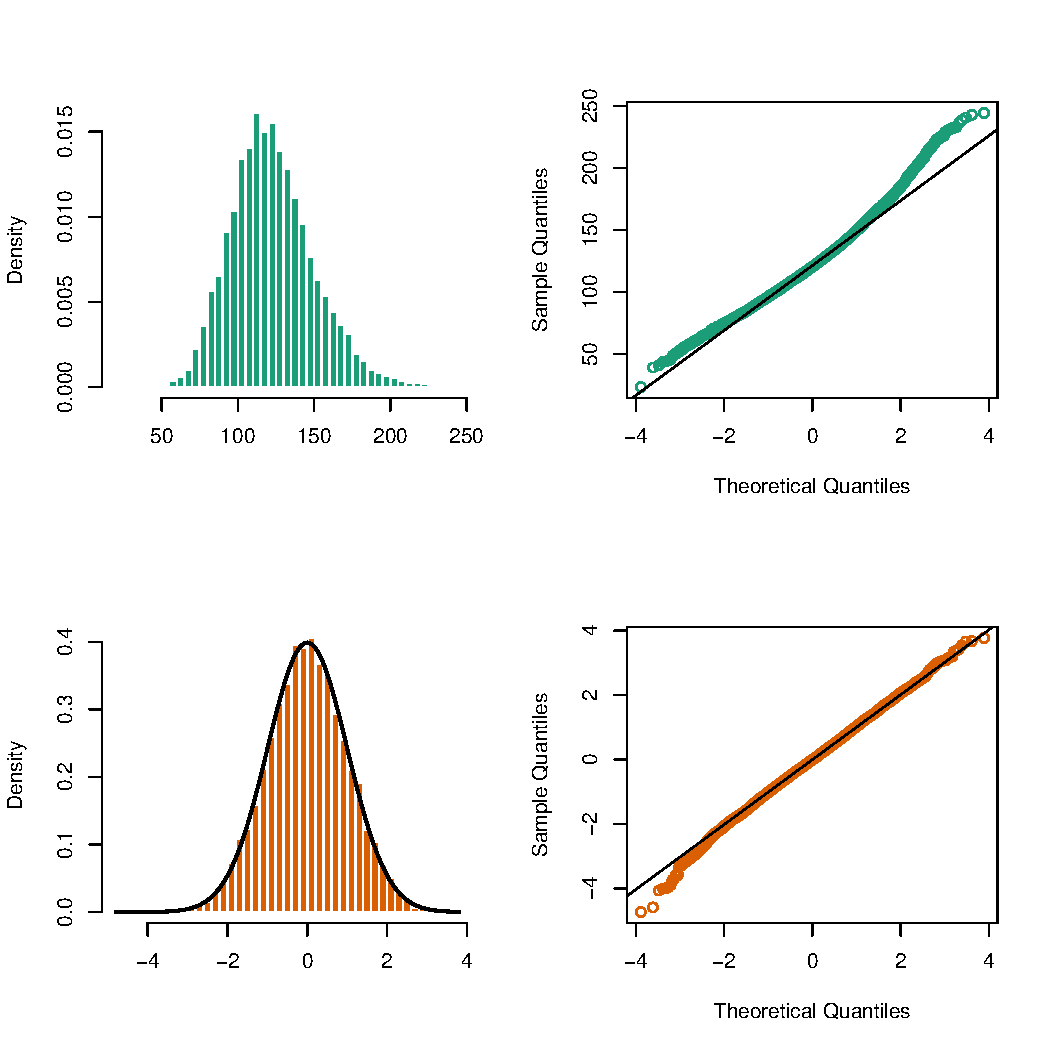
\includegraphics[width=\maxwidth]{figure/hist1} 

}

\caption[Histograms and normal Q-Q plots for the 9,999 bootstrap replicates of $\widehat{x}_0$ and $\mathcal{Q}$]{Histograms and normal Q-Q plots for the 9,999 bootstrap replicates of $\widehat{x}_0$ and $\mathcal{Q}$. \textit{Bottom}: Inverse estimator, $\widehat{x}_0$. \textit{Bottom}: Predictive pivot, $\mathcal{Q}$.\label{fig:hist1}}
\end{figure}


\end{knitrout}


%% Bibliography
\bibliographystyle{biom} \bibliography{supplementary}

\end{document}
